\section{Resultados de la evaluación reservada}
Las búsquedas completaron 3\,200 ajustes de validación: 200 de logística y 750 de cada otra familia. Se comprobaron los parámetros, las huellas de las predicciones, la cobertura de los pliegues y la reproducción de AP. Se conservaron 25 candidatos calibrados, uno por familia y corte. La familia principal elegida por validación fue XGBoost en los días 7, 28, 42 y 56, y Random Forest en el día 14. Estas decisiones quedaron congeladas antes de abrir la prueba.

La Tabla~\ref{res:principales} muestra el tamaño de cada población de prueba y la precisión promedio del candidato principal. Los intervalos se obtuvieron de los 2\,000 remuestreos previstos por personas. Las personas y las inscripciones se cuentan por corte; no deben sumarse entre cortes como si fueran individuos diferentes.
\begin{table}[!htbp]\centering
\caption{Población de prueba y AP de la familia principal; intervalos percentiles del 95\,\%.}\label{res:principales}
\begin{tabular}{rlrrrrl}
\toprule
Día & Familia & Inscr. & Personas & Retiros & AP & Intervalo\\
\midrule
7 & XGBoost & 5815 & 5211 & 1327 & 0,283 & [0,264; 0,303]\\
14 & Random Forest & 5610 & 5048 & 1116 & 0,233 & [0,216; 0,251]\\
28 & XGBoost & 5503 & 4968 & 1003 & 0,286 & [0,261; 0,314]\\
42 & XGBoost & 5400 & 4901 & 898 & 0,272 & [0,247; 0,299]\\
56 & XGBoost & 5302 & 4824 & 800 & 0,255 & [0,232; 0,285]\\
\bottomrule
\end{tabular}
\end{table}


La Figura~\ref{res:apfig} compara AP con la referencia constante, cuya AP coincide con la prevalencia de retiro en prueba. Los intervalos de las diferencias pareadas entre cada principal y la referencia quedaron por encima de cero en los cinco cortes: desde [0,040; 0,070] en el día 7 hasta [0,085; 0,129] en el día 56. Estos intervalos describen incertidumbre condicionada al paquete y a las ofertas observadas; no constituyen pruebas confirmatorias múltiples ni permiten ordenar los cortes por utilidad educativa.
\begin{figure}[!htbp]\centering
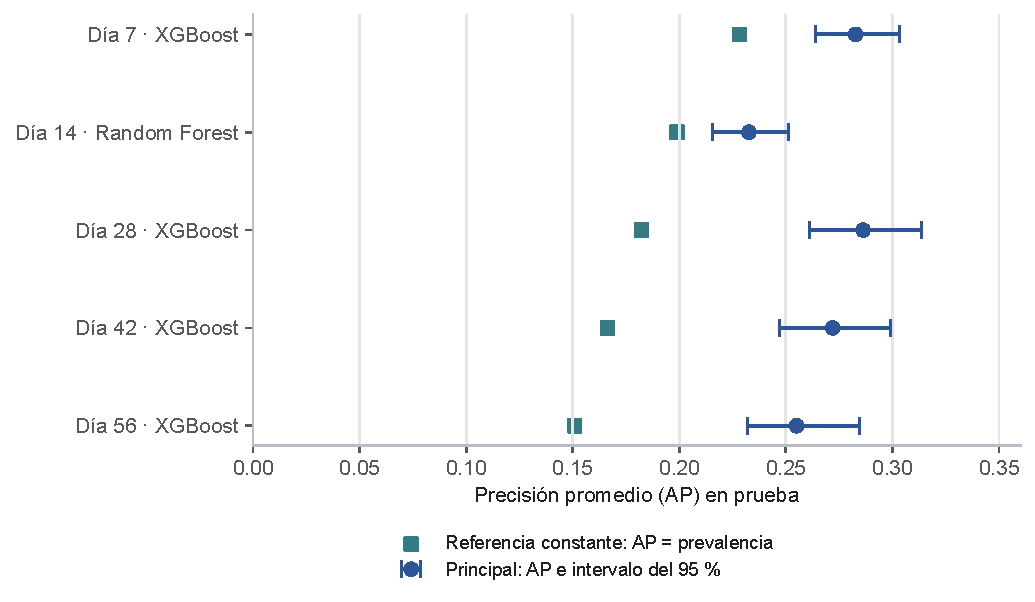
\includegraphics[width=\linewidth]{figuras_resultados/ap_principales.pdf}
\caption{AP en prueba del principal y referencia de prevalencia. Cada fila corresponde a una población y un horizonte distintos.}\label{res:apfig}
\end{figure}

La comparación entre familias de la Tabla~\ref{res:comparacion} muestra diferencias puntuales pequeñas en varios cortes. La principal seleccionada no obtiene siempre la AP más alta en prueba: al día 14 XGBoost alcanza 0,237 frente a 0,233 de Random Forest. Se conserva este resultado sin sustituir retrospectivamente a Random Forest. Los intervalos pareados de AP entre el principal y logística incluyen cero en los cinco cortes; por ello, no se sostiene una ventaja concluyente de los principales sobre logística a partir de estos intervalos. Tampoco se establece equivalencia entre algoritmos.
\begin{table}[!htbp]\centering
\caption{AP de los candidatos congelados en prueba. La mayor cifra no redefine al principal.}\label{res:comparacion}
\begin{tabular}{rrrrrr}
\toprule
Día & Logística & RF & LightGBM & XGBoost & TabNet\\
\midrule
7 & 0,278 & 0,281 & 0,283 & 0,283 & 0,275\\
14 & 0,232 & 0,233 & 0,234 & 0,237 & 0,235\\
28 & 0,280 & 0,284 & 0,290 & 0,286 & 0,264\\
42 & 0,269 & 0,272 & 0,274 & 0,272 & 0,257\\
56 & 0,244 & 0,262 & 0,260 & 0,255 & 0,248\\
\bottomrule
\end{tabular}
\end{table}


\section{Alertas, errores y anticipación}
La precisión es la proporción de alertas que corresponde a retiros posteriores; la sensibilidad es la proporción de retiros posteriores que el modelo detecta. La Tabla~\ref{res:alertas} permite leerlas junto con la proporción de inscripciones que recibiría una alerta. Los umbrales se eligieron en desarrollo para maximizar F1 y se mantuvieron sin cambios en prueba; no representan una capacidad institucional de atención acordada.
\begin{table}[!htbp]\centering
\caption{Clasificación en prueba con los umbrales congelados; alertas en porcentaje de inscripciones.}\label{res:alertas}
\begin{tabular}{rrrrrr}
\toprule
Día & Umbral & Precisión & Sensibilidad & F1 & Alertas (\%)\\
\midrule
7 & 0,206 & 0,259 & 0,726 & 0,382 & 64,0\\
14 & 0,188 & 0,229 & 0,695 & 0,344 & 60,4\\
28 & 0,201 & 0,299 & 0,357 & 0,325 & 21,8\\
42 & 0,145 & 0,222 & 0,688 & 0,336 & 51,5\\
56 & 0,165 & 0,255 & 0,440 & 0,323 & 26,0\\
\bottomrule
\end{tabular}
\end{table}


Al día 7 se alertaría sobre el 64,0\,\% de las inscripciones: se detectan 964 de los 1\,327 retiros futuros, pero 2\,756 alertas corresponden a inscripciones sin ese evento. La precisión es 25,9\,\%. Al día 28 se alertaría sobre el 21,8\,\%: se detectan 358 retiros y se omiten 645, con 841 falsas alertas. La mayor precisión de este corte no implica que detecte más retiros ni que sea una ventana óptima. En los principales, la precisión varía entre 22,2\,\% y 29,9\,\%; esa carga de falsas alertas limita una interpretación operativa favorable basada solamente en AP.

En la Tabla~\ref{res:anticipacion}, VP designa retiros correctamente alertados, FP alertas sin retiro posterior y FN retiros no alertados. La anticipación describe exclusivamente los VP: es la diferencia entre la fecha de retiro y el día de corte. Los cuartiles delimitan el 50\,\% central de esos tiempos; no son intervalos de confianza.
\begin{table}[!htbp]\centering
\caption{Errores y anticipación entre alertas correctas. Los cuartiles se expresan en días desde el corte hasta el retiro.}\label{res:anticipacion}
\begin{tabular}{rrrrrrr}
\toprule
Día & VP & FP & FN & Q25 & Mediana & Q75\\
\midrule
7 & 964 & 2756 & 363 & 18,0 & 61,5 & 135,2\\
14 & 776 & 2615 & 340 & 34,0 & 88,0 & 144,0\\
28 & 358 & 841 & 645 & 25,0 & 76,0 & 136,8\\
42 & 618 & 2163 & 280 & 30,0 & 74,0 & 125,0\\
56 & 352 & 1029 & 448 & 23,0 & 69,0 & 114,0\\
\bottomrule
\end{tabular}
\end{table}


Las medianas de anticipación varían entre 61,5 y 88 días. No significan que una intervención hubiera evitado el retiro ni describen a las personas no detectadas. Tampoco cambian de forma necesariamente ordenada entre cortes: varían la población, los retiros detectados y el horizonte restante de cada oferta.

\section{Probabilidades y límites de generalización}
La Tabla~\ref{res:calibracion} presenta ROC-AUC, que resume la ordenación de positivos frente a negativos, y Brier, el promedio del error cuadrático entre probabilidades y desenlaces. Una cifra menor de Brier representa menor error probabilístico. Los candidatos principales reducen Brier frente a la referencia constante, aunque la diferencia absoluta es pequeña; esto no demuestra por sí solo calibración perfecta ni una mejora atribuible exclusivamente al calibrador, pues no se realizó aquí una comparación base frente a calibrado.
\begin{table}[!htbp]\centering
\caption{Prevalencia, discriminación y error probabilístico en prueba del candidato principal.}\label{res:calibracion}
\begin{tabular}{rrrrr}
\toprule
Día & Prevalencia & ROC-AUC & Brier principal & Brier referencia\\
\midrule
7 & 0,228 & 0,590 & 0,1730 & 0,1761\\
14 & 0,199 & 0,570 & 0,1579 & 0,1594\\
28 & 0,182 & 0,634 & 0,1432 & 0,1490\\
42 & 0,166 & 0,649 & 0,1329 & 0,1386\\
56 & 0,151 & 0,667 & 0,1225 & 0,1281\\
\bottomrule
\end{tabular}
\end{table}


La Figura~\ref{res:calfig} contrasta la probabilidad media con la frecuencia observada de retiro en los intervalos no vacíos. La diagonal representa coincidencia. Los extremos con pocas observaciones deben leerse con cautela; los tamaños por intervalo se conservan con los resultados. La figura describe las probabilidades calibradas del paquete, sin ajustar una nueva calibración sobre la prueba.
\begin{figure}[H]\centering
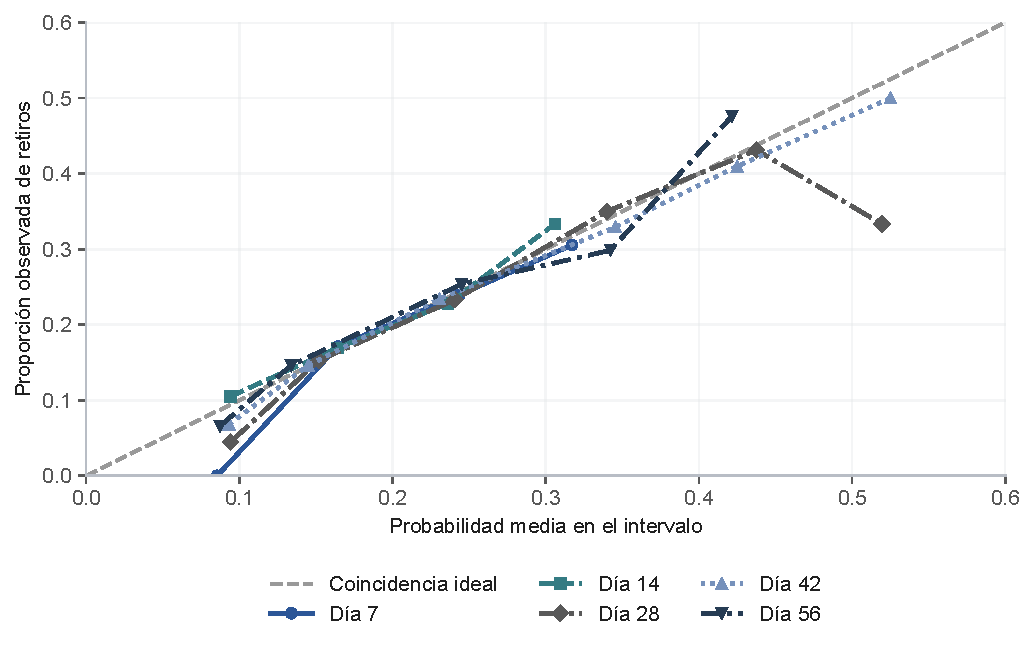
\includegraphics[width=\linewidth]{figuras_resultados/calibracion_principales.pdf}
\caption{Probabilidades y frecuencias observadas por intervalos fijos en los candidatos principales. Solo se representan intervalos con observaciones.}\label{res:calfig}
\end{figure}

Las salidas por oferta conservan inscripciones, personas, retiros y métricas descriptivas; no se utilizaron para seleccionar modelos ni umbrales. Los resultados estiman desempeño en personas nuevas dentro de ofertas ya representadas, no transportabilidad a periodos futuros o instituciones diferentes. Los intervalos por personas no incorporan la variabilidad de volver a entrenar los modelos o incorporar ofertas nuevas.

La exploración previa utilizó OULAD completo antes de la partición. Se mantiene como antecedente documentado; no se ha demostrado que se eligieran variables por mejorar la clasificación en la futura prueba. Desde la fijación del protocolo, la selección se restringió al desarrollo. La evaluación final no autoriza cambios para mejorar estas mismas cifras: cualquier nueva decisión basada en ellas sería exploratoria y requeriría otra evaluación independiente.

